\documentclass[a4paper]{article}

\usepackage[english]{babel}
\usepackage[utf8]{inputenc}
\usepackage{amsmath}
\usepackage{graphicx}
\usepackage[colorinlistoftodos]{todonotes}
\usepackage{titling}
\usepackage{listings}
\usepackage[T1]{fontenc}
\usepackage{array,multirow,makecell}
\setcellgapes{1pt}
\makegapedcells
\newcolumntype{R}[1]{>{\raggedleft\arraybackslash }b{#1}}
\newcolumntype{L}[1]{>{\raggedright\arraybackslash }b{#1}}
\newcolumntype{C}[1]{>{\centering\arraybackslash }b{#1}}

\newcommand{\subtitle}[1]{%
  \posttitle{%
    \par\end{center}
    \begin{center}\large#1\end{center}
    \vskip0.5em}%
}
\lstset{%
  basicstyle=\scriptsize\sffamily,%
  commentstyle=\footnotesize\ttfamily,%
  frameround=trBL,
  frame=single,
  breaklines=true,
  showstringspaces=false,
  numbers=left,
  numberstyle=\tiny,
  numbersep=10pt,
  keywordstyle=\bf
}





%%%%%%%%%%%%%%%%%%%%%%%%%%%%%%%%%%%%%%%%%%%%%%%%%%%%
% Raport Headers:
%%%%%%%%%%%%%%%%%%%%%%%%%%%%%%%%%%%%%%%%%%%%%%%%%%%%
\title{Image and signal processing: Computer exercise 3\\CE03G02T05}
\author{SID-LAKHDAR Riyane, PRULIERE Valentin}
\date{15/11/2015}

\begin{document}
% Beginning serious stuff.


\maketitle
% Actually prints title / subtitle / authors and dat into the document


%%%%%%%%%%%%%%%%%%%%%%%%%%%%%%%%%%%%%%%%%%%%%%%%%%%%
% Abstract
%%%%%%%%%%%%%%%%%%%%%%%%%%%%%%%%%%%%%%%%%%%%%%%%%%%%
\begin{abstract}
This report summarize, explains and refers to the answers we have designed for the third ''Image and Signal Processing'' computer exercise.\\
\end{abstract}

%%%%%%%%%%%%%%%%%%%%%%%%%%%%%%%%%%%%%%%%%%%%%%%%%%%%
% Introduction
%%%%%%%%%%%%%%%%%%%%%%%%%%%%%%%%%%%%%%%%%%%%%%%%%%%%
\section{Introduction}


The aim of the current computer exercise is to have a first theoretical and experimental approach with two systems often used in signal processing: The Fourier transform ($F$, and its inverse function $F^{-1}$) and the convolution.\\
The idea behind using these systems is to create a function space where the signals have properties which make them easier to study.  However, to use a property P on a signal in the output space, we need to explicitly identify how to transcript this property in the input space.\\

Thus, in the following study, we will try to show the main properties of the output signals of the two systems.  We will also try to transcript properties such as periodicity or time scaling from the output space of these systems to properties in them input space.   Finally, we will try to consider the time complexity of each system and see how to improve it using the mathematical properties of the two systems.\\

In this report, we have tried to separate as much as possible our theoretical researches from the output results of our programs, by implementing them regardless of the theoretical expectations.\\
In this purposes, we have designed the two following sections of this report:
\begin{itemize}
   \item ''Material \& Methods'': In this section, we described the theoretical methods used to answer to our different questions.  We provided the expected algorithms, their main principles or their python implementation.
   \item ''Experiments'': In this section, we gave the experimental results of our experiments.  We tried to explain them, and see whether they are consistent with the theoretical expectations or not.
\end{itemize}

\section{Material \& Methods}
    \subsection{Fourier transform}
        \subsubsection{Definition}
The Fourier transform of uni-dimensional function (usually of time) decomposes this input signal into the frequencies that make it up. This mathematical operator maps a function from the real space (depending on time) with a complex function (of frequency).   The main interest of this transform is that the absolute value of the transformed function represents the amount of cycles frequencies present in the original signal and complex argument of the transformed function is the phase offset of the basic sinusoid in that frequencies.   Thus, analyzing the time and frequency behavior of signals can be made easier by this transform. (\footnote{[ref: https://en.wikipedia.org/wiki/Fourier\_transform]}).\\







        \subsubsection{Formal definition and implementation on discrete time depending signals}
        For a given discrete uni-dimension signal s containing the N samples {s[0], ... s[N-1]}, the uni-dimensional discrete Fourier transform of s is defined for each input t of s as: $F(s)[t] = \sum_{k=0}^{N-1}{s[k]*\exp^{-2 i \pi k \frac{t}{N}}}$.\\
        To compute the Fourier transform of a discrete time-dependent signal, we have implemented the python function (fig \ref{1DFT.py}). We also have used  the same template to implement the inverse function of the Fourier transform (Fig \ref{1invDFT.py})
        \begin{figure}[ht!]
	    	\lstset{language=Python}
	     	\begin{lstlisting}
def myDFT1D(signal):
  length  = len(signal)
  i       = complex(0,1)
  res     = []
  for muInd in range(0, length):
      currRes  = 0
      for xInd in range(0, length):
          currRes  += signal[xInd] *  np.exp(-i * 2 * np.pi * muInd * xInd / length)
      res.append(currRes)
  return res
            \end{lstlisting}
            \caption{Python code to compute Fourier transform of a time depending discrete signal.}
		    \label{1DFT.py}
	    \end{figure}

        \begin{figure}[ht!]
	    	\lstset{language=Python}
	     	\begin{lstlisting}
def myInvDFT1D(ft):
    length  = len(ft)
    i       = complex(0,1)
    res     = []
    for tInd in range(0, length):
        currRes  = 0
        for muInd in range(0, length):
            currRes += ft[muInd] * np.exp(i * 2 * np.pi * tInd * muInd / length)
        res.append(currRes / length)
    return res

            \end{lstlisting}
            \caption{Python code to compute the inverse function of the Fourier transform.}
		    \label{1invDFT.py}
	    \end{figure}
        
        The proper functioning of these two functions will be shown in the Experiments section using some input signals and the theoretically known transform (such as an impulse or a Gaussian signal).  We will also check if some basic properties of the Fourier transform are respected by our programs (such as $f(t) = FT^{-1}(FT(f(x)))$).

        
        
        
        
        
        
        
        
        
	\subsubsection{Advantages and properties}
        Thanks to the uni-dimension Fourier transform previously defined, we are able to:
        \begin{itemize}
	    \item Make a mapping between a given uni-dimensional signal in the real domain and a function of the complex domain.
            \item This map exists for any uni-dimensional input signal (\footnote{Here we suppose that this signal is an integrable functions, or Lebesgue-measurable: $\int_{-\infty}^{\infty}{|f(x)| dx} < \infty$}) and is unique.
	\end{itemize}
        The first interest of this transform is that the transformed function is a complex function.  Thus, it has many forms which can be used depending on the studied case:
        \begin{itemize}
	    \item A Eulerian form (composed of sinus and a cosinus function) which is more suitable for studying the periodic behavior of our signal over time or frequency.  As we know the bounds of the sinus and cosinus functions, this form is also very useful to determine the bounds of our signal's components.
	    \item An exponential form (composed of an amplitude and a phase) which allows to write multiplication signals thanks to simple phase additions.
	\end{itemize}
        Secondly, the Fourier transform is a linear application.    Thus, study a signal $s(x) = \alpha_{0}s_{0}(x) + \alpha_{1}s_{1}(x)$ through its Fourier transform is equivalent to study the Fourier transform of $s_{0} and s_{1}$ which may be easier.   This is the main property we will use to study convolutions in the following sections.\\
        
        Finally the time (and frequency) property we can notice on the transformed function may be directly transcribed on time (and frequency) properties for the initial real function, using mapping that we will show for specific signals.
        
        
        
        
    \subsection{First use of the Fourier transform: discrete impulse signal}
    	\subsubsection{Formal expression of the Fourier transform}
	Let consider the impulse function
	\begin{equation*}
	\delta_{a} : x \rightarrow \delta(x - a) = \left\{
		    \begin{array}{l l}
			    1 ; \textrm{ if } x = a\\
			    0 ; \textrm{ otherwise }\\
		    \end{array} \right.
	\end{equation*}
	Using the definition of the Fourier transform, we have:
	\begin{equation}
	\begin{aligned}
		F(\delta_{a})[\omega] = \delta_{a}[\omega]
	    &= \sum_{k=-\infty}^{+\infty}{\delta_{a}[k]*\exp^{-2 i \pi \omega k}} \\
	    &= \sum_{k=-\infty, k\neq a}^{+\infty}{\delta_{a}[k]*\exp^{-2 i \pi \omega k}} + \delta_{a}[a]*\exp^{-2 i \pi \omega a} \\
	    &= \exp^{-2 i \pi \omega a}
	\end{aligned}
	\end{equation}
	Using this expression, we can deduce the Fourier transform of the impulse signal using the following forms:\\
	The Eulerian form of the exponential transform: $\delta_{a}[\omega] = cos(-2 i \pi \omega a) + i sin(-2 i \pi \omega a)$.   Thus
	\begin{equation*}
    \begin{aligned}
	    (Re \Delta_{a})[\omega] &= cos(-2 \pi a \omega) = cos(2 \pi a \omega)\\
	    (Im \Delta_{a})[\omega] &= sin(-2 \pi a \omega) = -sin(2 \pi a \omega)\\
	\end{aligned}
	\end{equation*}
	We can also use the exponential form of the Fourier transform to deduce
	\begin{equation*}
    \begin{aligned}
	    (Mag \Delta_{a})[\omega] &= 1\\
	    (Phase \Delta_{a})[\omega] &= (-2 \pi a \omega) mod 2 \pi\\
	\end{aligned}
	\end{equation*}
	
	To have an experimental approach of this results, we have implemented the python function given at the figure Fig \ref{generateDelta.py} which generates an impulse signal $\delta_{a}$.
        \begin{figure}[ht!]
	    \lstset{language=Python}
	    \begin{lstlisting}
def generateDelta(IdxSampleWhereImpuls, numberOfSamples):
    res = [0 for j in xrange(numberOfSamples)]
    res[IdxSampleWhereImpuls] = 1
    return res
            \end{lstlisting}
            \caption{Python code to generate an impulse signal $\delta_{a}$.}
	    \label{generateDelta.py}
	\end{figure}
	In the next section, we will use this function to experimentally check the previous results.





	
        \subsubsection{Impact on the decomposition of the signal: periodicity}
        Using the previous expressions of the Fourier transform, we can notice that the real and the imaginary part of the Fourier transform are periodic with the same period = a.
        Thus, a time shifting in the input impulse function (changing the value of a) results in a time scaling (frequency change) in the transformed function.

        
        
        
        
        
        
        
    \subsection{Convolution and derivative expressions}
    	In the previous section, we have studied how time shifting and time scaling of an input signal may influence the output signal of a system (Fourier transform system).   Let's now study an other system: the convolution system(s).   The main topic of this section will be to determine the impact of the length of causal signals on them transform.   We will also see how and why to use a Fourier transform to compute a convolution and describe a signal. Finally, we will see the limits of this method (in the Experiments section).
        \subsubsection{Linear and circular convolution definition}
        The linear and circular convolutions of two causal input function x and y, of length $N_{x} and N_{y}$ are defined by:
        \begin{equation*}
        \begin{aligned}
			z_{lin}[k] &= \sum_{l=0}^{k}{x[l]*y[k-l]}\\
            z_{circ}[k] &= \sum_{l=0}^{k}{x[l]*y[(k-l)mod M]}
        \end{aligned}
		\end{equation*}
        The M that appears in circular convolution's equation will be the parameter that we will variate to show the properties of this convolutions.\\
		To compute the circular convolution of two input signals, we have designed the python program given by the figure Fig \ref{circularConvolution.py}
        \begin{figure}[ht!]
          \lstset{language=Python}
          \begin{lstlisting}
def my1DCircularConvolution(x, y, M):
    Nx  = len(x)
    Ny  = len(y)
    # Creates a M size copy of x and y where filled with zero at the end
    x_M = copy_and_fill_with_zero(x, M)
    y_M = copy_and_fill_with_zero(y, M)
    z   = []
    for k in xrange(M):
        resK = 0
        for l in xrange(M):
			resK += x_M[l] * y_M[(k-l)%M]
		z.append(resK)
    return z
            \end{lstlisting}
            \caption{Python code to generate a circular convolution.}
	    \label{circularConvolution.py}
		\end{figure}
        
        \subsubsection{Circular convolution using Fourier transform}
        The program Fig \ref{circularConvolution.py} computes a circular convolution with a complexity $O(N^{2})$.  But we know that the circular convolution may be computed using the Fourier transform as follows $z_{circ}[k] = F^{-1}(F(x[k])[n] * F(y[k])[n])$.  As we know that the Fourier transform of a signal of length N may be computed with a complexity O(N log(N)), we can provide the program figure Fig \ref{circularConvolutionUsingFourier.py} which will compute a circular convolution in a more efficient way than the one Figure Fig \ref{circularConvolution.py}
        \begin{figure}[ht!]
          \lstset{language=Python}
          \begin{lstlisting}
def my1DCircularConvolution_fourier(x, y, M):
    # Creates a M size copy of x and y where filled with zero at the end
    x_M  = copy_and_fill_with_zero(x, M)
    y_M  = copy_and_fill_with_zero(y, M)
    TF_x = myDFT1D(x_M)
    TF_y = myDFT1D(y_M)
    return myInvDFT1D(myProd(TF_x, TF_y))
            \end{lstlisting}
            \caption{Python code to efficiently generate a circular convolution using a Fourier transform.}
	    \label{circularConvolutionUsingFourier.py}
		\end{figure}





\section{Experiments}
    \subsection{Fourier transform and inverse}
	    In this section, we will consider the programs we designed to compute the Fourier transform and its inverse functions (Fig \ref{1DFT.py} and Fig \ref{1invDFT.py}).   We will try to show their proper functioning using some theoretically known properties on the Fourier transform applied on Gaussian function and an impulse function.
    	\subsubsection{Check basic property of the Fourier transform}
	    The first Fourier transform property we will use is: for each uni-dimension signal f and for each input of f, $f(t) = FT^{-1}(FT(f(x)))$.\\
            \begin{figure}[!htb]\centering
                \begin{minipage}{0.45\textwidth} \frame{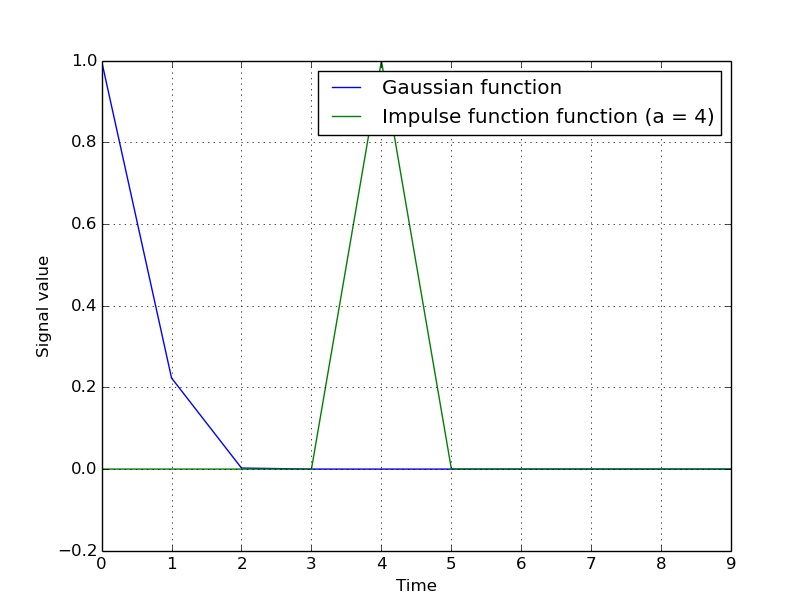
\includegraphics[width=\linewidth]{gaussianAndImpulse.png}} \end{minipage}
                \begin{minipage}{0.45\textwidth} \frame{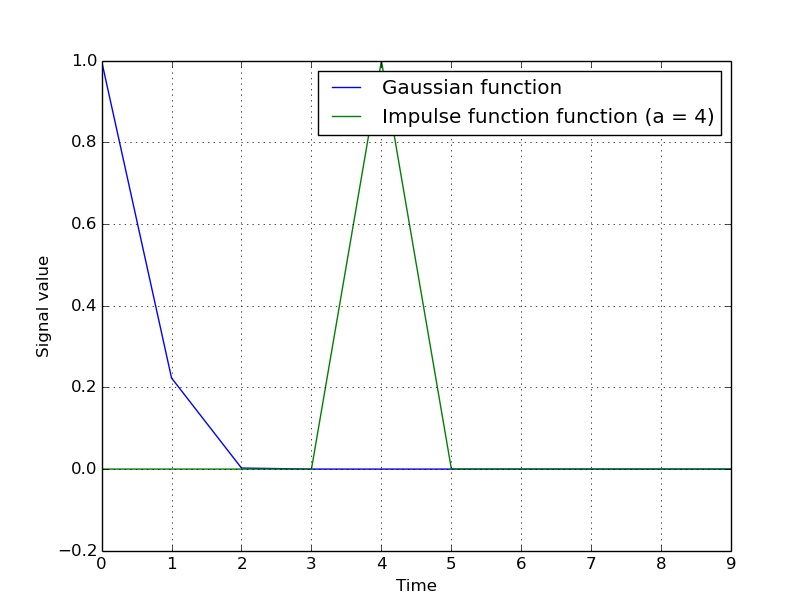
\includegraphics[width=\linewidth]{gaussianAndImpulse.png}} \end{minipage}
                \caption{Gaussian and impulse signal on the left.  $FT^{-1}(FT(f(x)))$ on the right}
                \label{gaussianAndImpulse.png}
			\end{figure}

            
            We can notice on the figure Fig \ref{gaussianAndImpulse.png} that our program respect this property for the input signals $f(x) = \exp^{1.5 * x^{2}}$ (Gaussian) and $f(x) = 1 \mbox{ if }x = 4\mbox{ and } 0 \mbox{ otherwise}$.\\
            
            An other way to check the proper functioning of our program is to uses the theoretically known result: $F(gaussian)(\alpha) = F(\exp^{-A * x^{2}})(\alpha) = \exp^{\frac{-\pi^{2} * \alpha^{2}}{A}}  * \sqrt{\frac{\pi}{A}}$  (the proof may be obtained by simply applying the definition of the Fourier transform to the Gaussian function).   The figure Fig \ref{gaussianTransform.png} shows the Fourier transform of a Gaussian function obtained by our program.   We can notice on this figure the matching between the Fourier transform computed by our program and the expected function.\\
            \begin{figure}[!htb]\centering
                \begin{minipage}{0.45\textwidth} \frame{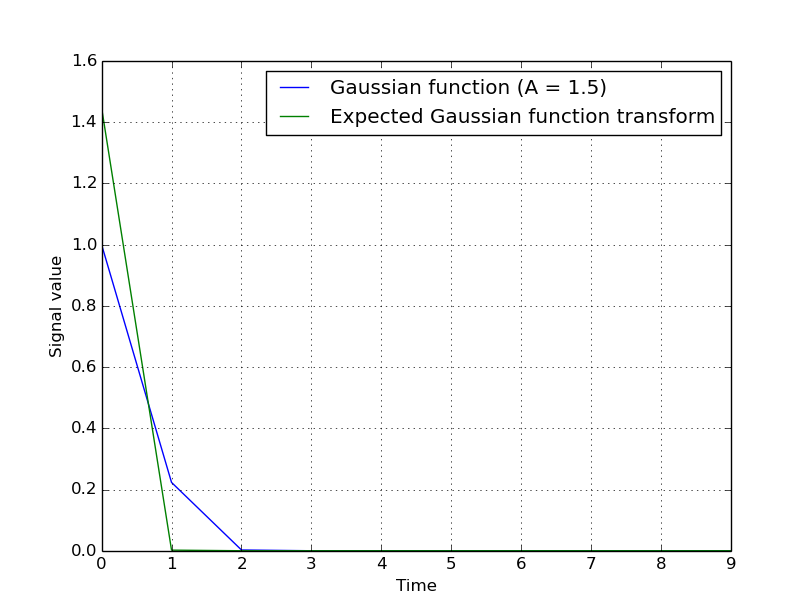
\includegraphics[width=\linewidth]{expectedGaussianTransform.png}} \end{minipage}
                \begin{minipage}{0.45\textwidth} \frame{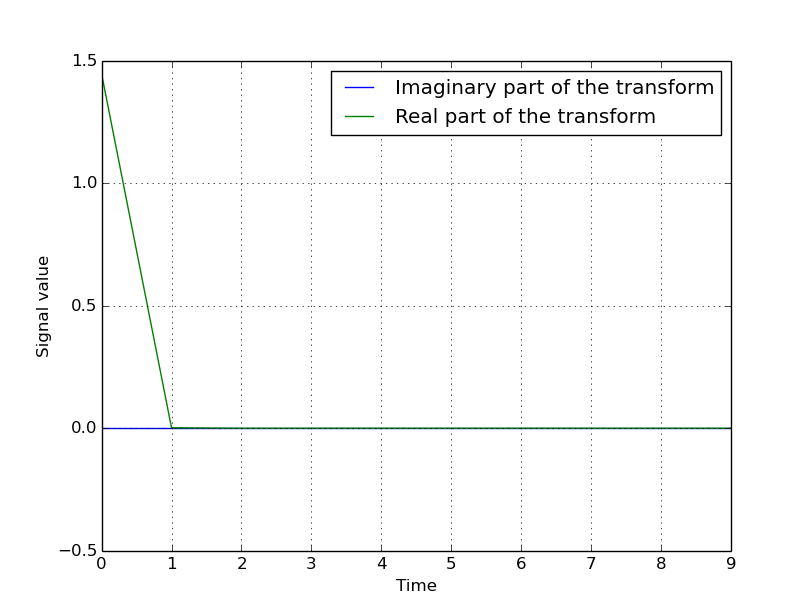
\includegraphics[width=\linewidth]{gaussianTransform.png}} \end{minipage}
                \caption{Theoretical and computed transform of a Gaussian.}
                \label{gaussianTransform.png}
			\end{figure}
            
            
            
            
            
            
	\subsubsection{Property of the Fourier transform on discrete impulse signals}
	Using the program defined previously, we will verify some properties on the Fourier transform of an impulse signal.\\
	First of all, the two first plots of the figure Fig \ref{ftDelta.png} represents the Fourier transform of the impulse signal where the non null value is in 0.   It confirms that if the non null value of the impulse is in 0, the Fourier transform of the signal is the constant integer 1.
    \begin{figure}[!htb]\centering
	    \begin{minipage}{0.45\textwidth} \frame{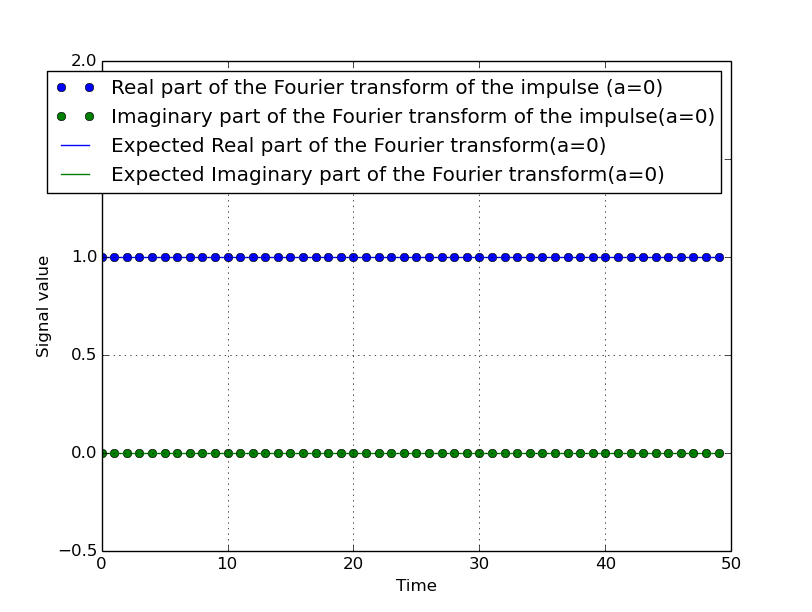
\includegraphics[width=\linewidth]{ft_Impulse0_re_im.png}} \end{minipage}
	    \begin{minipage}{0.45\textwidth} \frame{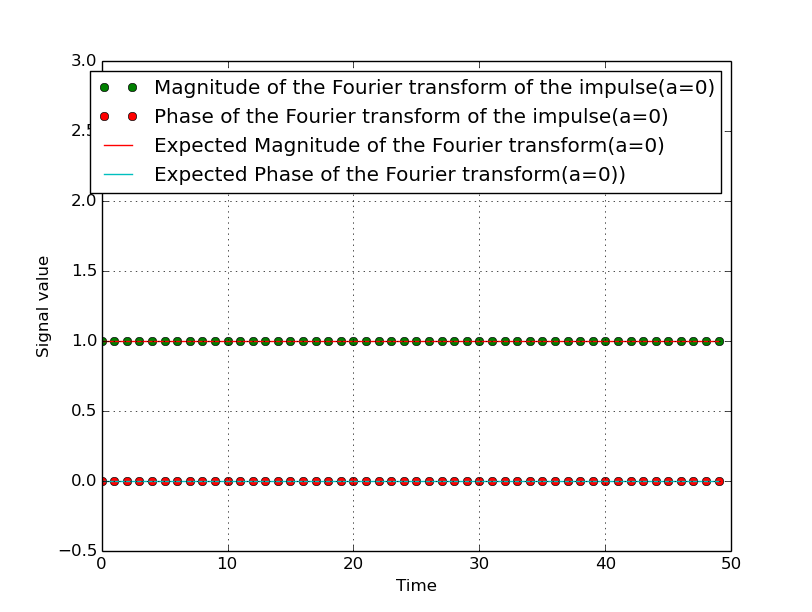
\includegraphics[width=\linewidth]{ft_Impulse0_mag_phase.png}} \end{minipage}
	    \begin{minipage}{0.45\textwidth} \frame{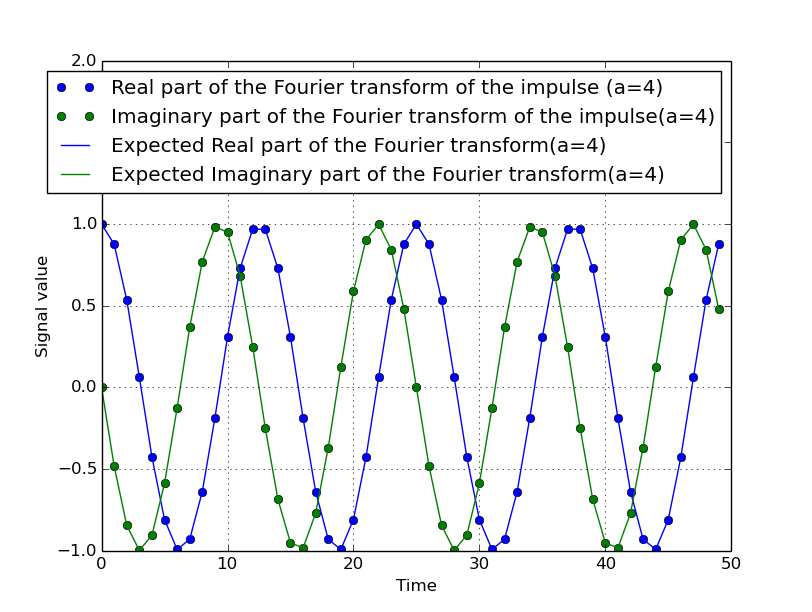
\includegraphics[width=\linewidth]{ft_Impulse4_re_im.png}} \end{minipage}
        \begin{minipage}{0.45\textwidth} \frame{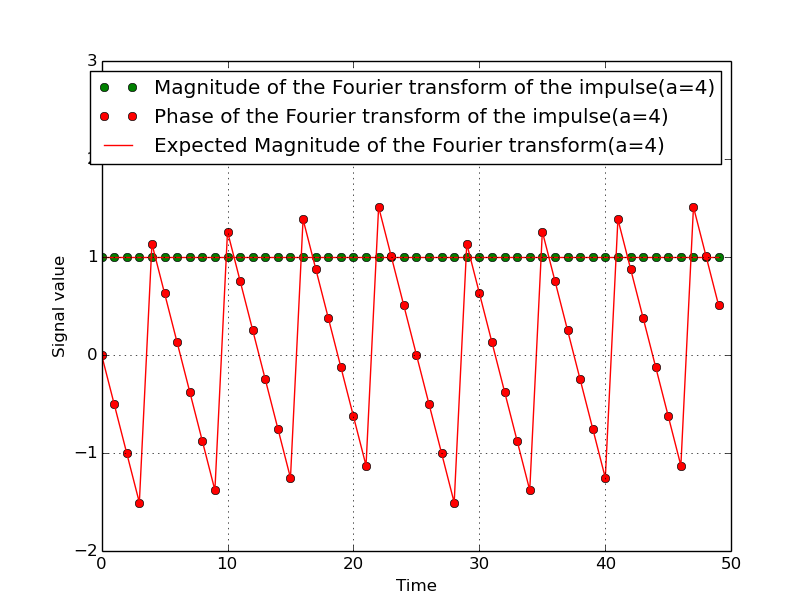
\includegraphics[width=\linewidth]{ft_Impulse4_mag_phase.png}} \end{minipage}
	    \begin{minipage}{0.45\textwidth} \frame{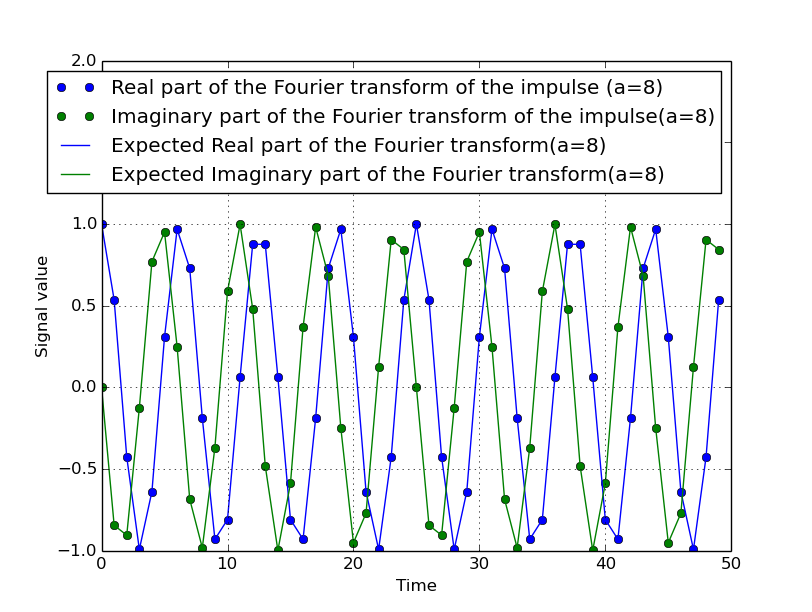
\includegraphics[width=\linewidth]{ft_Impulse8_re_im.png}} \end{minipage}
        \begin{minipage}{0.45\textwidth} \frame{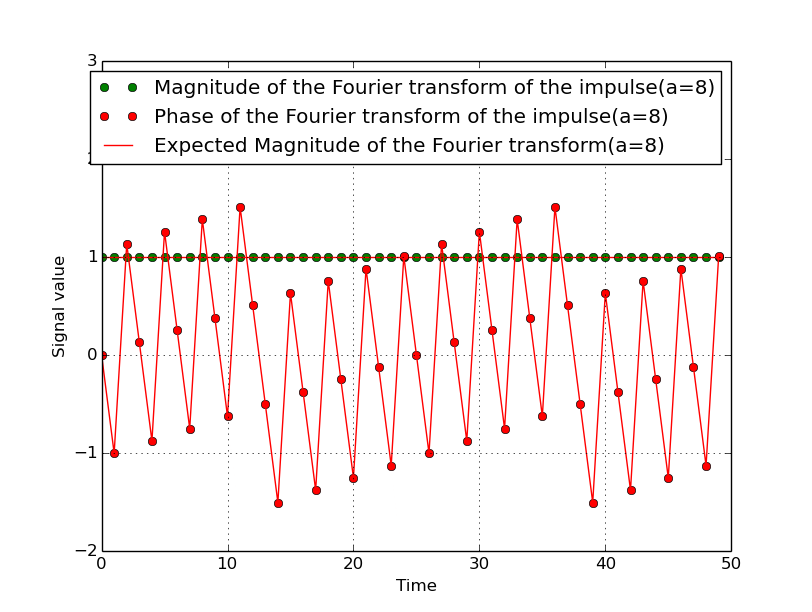
\includegraphics[width=\linewidth]{ft_Impulse8_mag_phase.png}} \end{minipage}
	    \caption{Fourier transform of $\delta_{0}, \delta_{4} and \delta_{8}$.}
	    \label{ftDelta.png}
    \end{figure}
    By changing the value of the non null index from 0 to 4 or to 8 (four last plots of the figure Fig\ref{ftDelta.png}), we can also confirm the good behavior of our program by comparing the computed value of the transform (dots) to the theoretically expected values(curves).   All this figures also allow us to confirm the periodic property of the Fourier transform of the impulse signal.  Finally, this figures allow us to confirm the link between the time shifting of the input impulse signal and the time scaling of the transform signal (the period of the transformed signal equals the shifting a of the initial signal $\delta_{0}$).

    



  


	\subsection{Convolution and Fourier transform}
    	\subsubsection{Use of the output signal length M}
        Let consider the two signals x = {5,1,2,6,4}, and y={1,2,3}.  Depending on the value of the length M of the output signal, the linear and circular convolution of x and y are:
        \begin{itemize}
			\item $M = N_{x} + N_{y} - 1$:\\
                \begin{tabular}{| L{2cm} || C{1cm} | C{1cm} | C{1cm} | C{1cm} | C{1cm} | C{1cm} | C{1cm} |}
                  \hline k & 0 & 1 & 2 & 3 & 4 & 5 & 6\\
                  \hline $z_{lin}$ & 5 & 11 & 19 & 13 & 22 & 26 & 12\\
                  \hline
                \end{tabular}
			\item $M = N_{x} + N_{y} - 1$:\\
                \begin{tabular}{| L{2cm} || C{1cm} | C{1cm} | C{1cm} | C{1cm} | C{1cm} | C{1cm} | C{1cm} |}
                  \hline k & 0 & 1 & 2 & 3 & 4 & 5 & 6\\
                  \hline $z_{circ}$ & 5 & 11 & 19 & 13 & 22 & 26 & 12\\
                  \hline
                \end{tabular}
			\item $M = max(N_{x}, N_{y})$:\\
                \begin{tabular}{| L{2cm} || C{1cm} | C{1cm} | C{1cm} | C{1cm} | C{1cm} |}
                  \hline k & 0 & 1 & 2 & 3 & 4\\
                  \hline $z_{circ}$ & 31 & 23 & 19 & 13 & 22\\
                  \hline
                \end{tabular}
		\end{itemize}

        
        
        
		\subsubsection{Equivalence between Fourier transform and linear convolution}
        The figure fig \ref{linear_circular_convolution_example.jpg} (left plot) allows us to see that our experimental results match the results we have calculated in the previous section.
        \begin{figure}[!htb]\centering
        \begin{minipage}{0.45\textwidth} \frame{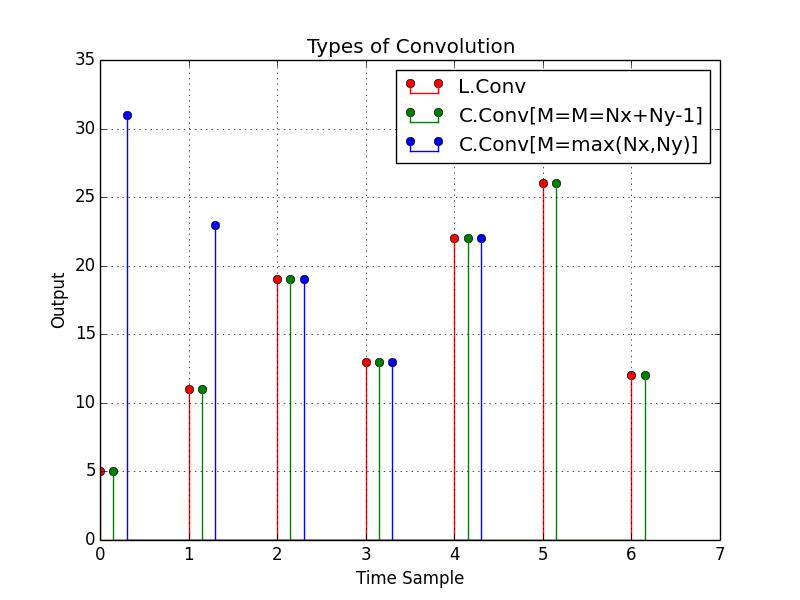
\includegraphics[width=\linewidth]{linear_circular_convolution_example.jpg}} \end{minipage}
        \begin{minipage}{0.45\textwidth} \frame{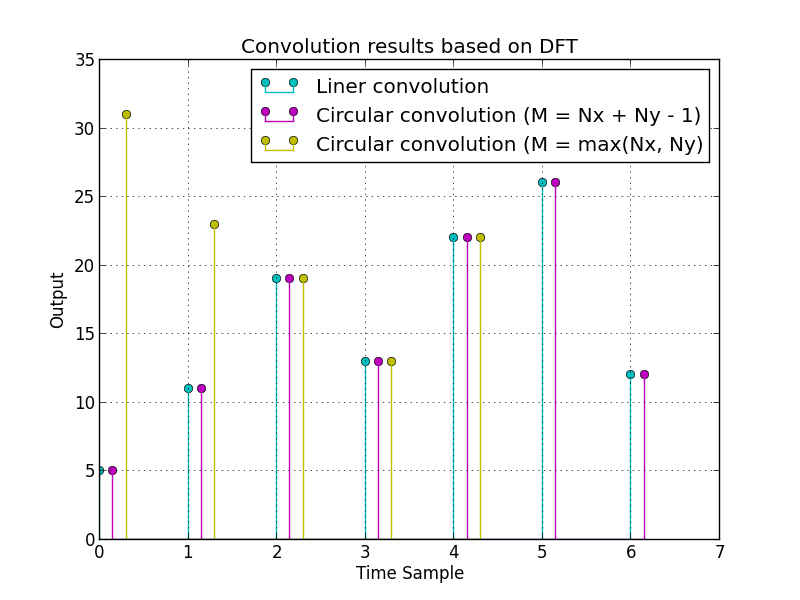
\includegraphics[width=\linewidth]{convDFT.png}} \end{minipage}
        \caption{Linear and circular convolution and them Fourier transform.}
        \label{linear_circular_convolution_example.jpg}
        \end{figure}\newline
        It also shows that the linear convolution is equivalent to the circular convolution when $M = N_{x} + N_{y} - 1$




\section{Conclusion}
During this computer exercise, we have described two ways to analyze the time and frequency behavior of a signal.   Thus, we can now conclude about the advantages of using the Fourier transform for analyzing an impulse signal, and its interesting time complexity compared to the convolution.
\end{document}
